\documentclass[class=report, crop=false, 12pt,a4paper]{standalone}
\usepackage{enumitem}
\usepackage{multicol}
\usepackage{etoolbox}
\AtBeginEnvironment{quote}{\singlespacing\small}
\usepackage{setspace}
\onehalfspacing
\usepackage{graphicx}
\usepackage{float}
\usepackage{amsmath}
\usepackage{amssymb}
\usepackage{siunitx}
\sisetup{detect-all}
\begin{document}
\section{Gas power cycles}
\subsection{Thermodynamic cycles}
Two important areas of application of thermodynamics are power generation and refrigeration. Both are accomplished by systems that operate on a thermodynamic cycle.
\begin{itemize}[noitemsep]
  \item Power cycles: operated as engines.
  \item Refrigeration cycles: operated as refrigerators, air conditioners, heat pumps, etc.
  \item Gas cycles: the working fluid remains in the gaseous phase throughout the entire cycle.
  \item Vapour cycles: the working fluid exists in the vapour phase during part of the cycle and in the liquid phase during another part. 
  \item Closed cycles: the working fluid is returned to the initial state at the end of the cycle and is recirculated.
  \item Open cycles: the working fluid is renewed at the end of the cycled instead of being recirculated.
\end{itemize}
\subsection{Heat engines}
In automobile engines, the combustion gases are exhausted and replaced by the fresh air-fuel mixture at the end of each cycle. The engine operates on a mechanical cycle but the working fluid does not go through a complete thermodynamic cycle. 
\begin{itemize}[noitemsep]
  \item Internal combustion engine: heat is supplied by burning the fuel within the system boundaries e.g. automobile engines.
  \item External combustion engine: heat is supplied to the working fluid from an external source such as a furnace e.g. steam power plants.
\end{itemize}
\subsection{Basic considerations in the analysis of power cycles}
The cycles encountered in actual devices are difficult to analyse because of the presence of complicating effects such as friction and the absence of sufficient time for establishment of the equilibrium conditions during the cycle. Thus, we utilise some idealisations. An ideal cycle is an actual cycle stripped of all its internal irreversibilities, producing a graph made up totally of internally reversible processes. The ideal cycle can be used to show the general characteristics. Recall,
\begin{align}
  \eta_{th} &= \frac{W_{net}}{Q_{in}} \textrm{ or}\\
  \eta_{th} &- \frac{w_{net}}{q_{in}} 
\end{align}
\begin{figure}[h]
  \centering
  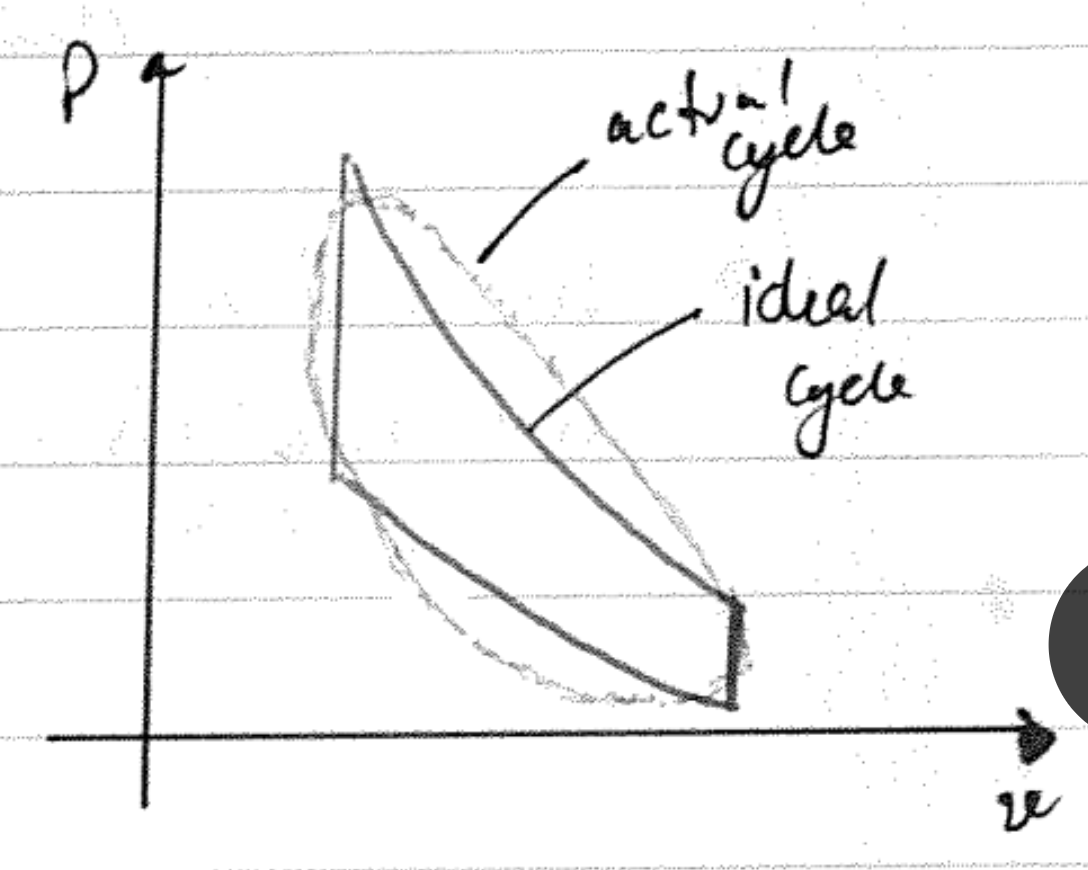
\includegraphics[width = 0.5\textwidth]{../img/actualvsidealcycle}
  \caption{How an ideal cycle compares to the actual cycle.}
  \label{fig:actualvsidealcycle}
\end{figure}
Also, heat engines on a totally reversible cycle (such as the Carnot cycle) have the highest thermal efficiency of all heat engines operating between the same temperature levels. The question arises: why do we not use the Carnot cycle? This is due to hardware. It is difficult to implement it. Thus, other ideal cycles are used.
\begin{equation}
  \eta_{th, \textrm{ totally reversible}} > \eta_{th, \textrm{ internally reversible}} = \eta_{th, \textrm{ ideal gas}}
\end{equation}
This applies between the same temperature limits. We also have:
\begin{equation}
  \eta_{th, \textrm{ ideal cycle}} > \eta_{th, \textrm{ actual cycle}}
\end{equation}
The idealisations and simplifications commonly employed in the analysis of power cycles can be summarised as follows:
\begin{enumerate}[noitemsep]
  \item The cycle does not involve any friction. Thus, the working fluid does not experience any pressure drop as it flows in pipes or devices such as heat exchangers.
  \item All expansion and compression processes take place in a quasi - equilibrium manner.
  \item The pipes connecting various components of a system are well insulated and heat transfer through them is negligible.
\end{enumerate}
Kinetic energy and potential energy are also generally neglected as their changes are negligible.
\begin{align}
  \textrm{KE and PE neglected for} & \begin{cases}
    \textrm{turbines}\\
    \textrm{compressors}\\
    \textrm{pumps}
  \end{cases}\\
  \textrm{KE neglected for} & \begin{cases}
    \textrm{condensers}\\
    \textrm{boilers}\\
    \textrm{mixing chambers}
  \end{cases}\\
  \textrm{KE not neglected for} & \begin{cases}
    \textrm{nozzles}\\
    \textrm{diffusers}
  \end{cases}
\end{align}
Also, note that for P-V and T-S diagrams, the area enclosed, for both, is the net work produced during a cycle.
\subsection{T-S diagram tips and tricks}
\begin{itemize}[noitemsep]
  \item A heat - addition process proceeds in the direction of increasing entropy. 
  \item A heat - rejection process proceeds in the direction of decreasing entropy. 
  \item An isentropic (internally reversible, adiabatic) process proceeds at constant entropy. 
  \item The area under the process curve on a T-S diagram represents the heat transfer for that process.
\end{itemize}
\subsection{The Carnot cycle and its value in engineering}
\begin{equation}
  \eta_{th, \textrm{ Carnot}} = 1 - \frac{Q_L}{Q_H} = 1 - \frac{T_L}{T_H}
  \label{carnotefficiency}
\end{equation}
Thermal efficiency increases with an increase in the average temperature at which heat is supplied to the system, or with a decrease in the average temperature at which heat is rejected from the system. The highest temperature in the cycle is limited by the maximum temperature that the components of the heat engine, such as the piston or the turbine blades, can withstand. The lowest temperature is limited by the temperature of the cooling medium utilised in the cycle such as a lake, a river or the atmospheric air.
\subsubsection{Proof question}
Show that the thermal efficiency of a Carnot cycle operating between the temperature limits $T_H$ and $T_L$ is solely a function of these two temperature and is given by equation \ref{carnotefficiency}.

Carnot cycle is:
\begin{enumerate}[noitemsep]
  \item Isothermal heat addition.
  \item Isentropic expansion.
  \item Isothermal heat rejection.
  \item Isentropic compression.
\end{enumerate}
\begin{figure}
  \centering
  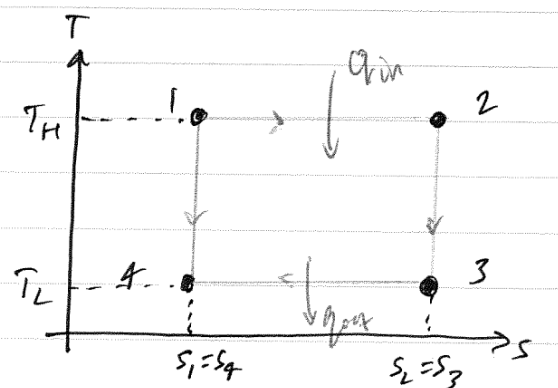
\includegraphics[width = 0.5\textwidth]{../img/carnotq}
  \caption{T-S diagram for Carnot cycle}
\end{figure}
\begin{align}
  q_{in} &= \textrm{Area under graph as processes are totally reversible}\\
  &= T_H(S_2 - S_1) = T_H(S_3 - S_4)\\
  q_{out} &= \textrm{Area under process 3-4}\\
  &= T_L(S_3 - S_4) = T_L(S_2 - S_1)\\
  \eta_{th} &= 1 - \frac{q_{out}}{q_{in}} = 1 - \frac{T_L(S_2 - S_1)}{T_H(S_2 - S_1)}\\
  \eta_{th, \textrm{ const}} &= 1 - \frac{T_L}{T_H}
\end{align}
\subsection{Air-standard assumptions}
Even though internal combustion engines operate on a mechanical cycle (the piston returns to its starting position at the end of each revolution), the working fluid does not undergo a complete thermodynamic cycle. It is thrown out of the engine at some point in the cycle (as exhaust gases) instead of being returned to its initial state. Working on an open cycle is the characteristic of all internal combustion engines. To reduce the analysis to a manageable level, we utilise the following approximations, commonly known as the \emph{air-standard assumptions.} Those cycles that run this are called air-standard cycles.
\begin{enumerate}[noitemsep]
  \item The working fluid is air, which continuously circulates in a closed loop and always behaves as an ideal cycle.
  \item All the processes are internally reversible.
  \item The combustion process is replaced by heat-addition process from an external source.
  \item The exhaust process is replaced by a heat rejection process that restores the working fluid to its initial state.
\end{enumerate}
Also we assume that air has constant specific heats whose value is determined at room temperature (25\si{\celsius}). When this assumption is applied, true air-standard assumptions are called the cold-air-standard assumptions.
\subsection{An overview of reciprocating engines}
The basic components of a reciprocating engine are shown in the diagrams.
\begin{figure}
  \centering
  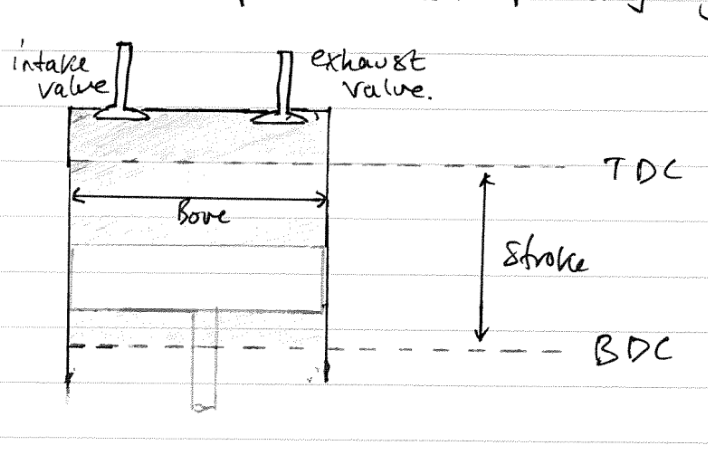
\includegraphics[width = \textwidth]{../img/ReciprocatingEngineDiagram}
  \caption{Basic components of a reciprocating engine.}
\end{figure}
\begin{itemize}[noitemsep]
  \item TDC: top dead center - position of the piston where it forms the smallest volume.
  \item BDC: bottom dead center - position of the piston where it forms the largest volume.
  \item Stroke: distance between TDC and BDC.
  \item Bore: diameter of the piston (internal diameter of the cylinder).
  \item Clearance volume: minimum volume formed.
  \item Displacement volume: the volume displaced by the piston as it moves between TDC and BDC.
\end{itemize}
The ratio of the maximum volume formed in the cylinder to the (minimum) clearance volume is called the compression ratio, r, of the engine.
\begin{gather}
  \textrm{Compression ratio: } r = \frac{V_{max}}{V_{min}} = \frac{V_{BDC}}{V_{TDC}}\\
  \textrm{Displacement volume} = \textrm{no. of cylinders} \times \textrm{stroke length} \times \textrm{bore area}
\end{gather}
The MEP (mean effective pressure) is a constant theoretical pressure, that if it acts on the piston to produce work, it would produce the same amount as that during an actual cycle. 
\begin{gather}
  \therefore W_{net} = \textrm{MEP} \times \textrm{piston area} \times \textrm{stroke}\\
  \textrm{or } W_{net} = \textrm{MEP} \times \textrm{displacement volume}\\
\end{gather}
or rearranging for MEP gives:
\begin{equation}
  \textrm{MEP} = \frac{W_{net}}{(V_{max} - V_{min})} = \frac{w_{net}}{(v_{max} - v_{min})}
\end{equation}
Engines with larger MEP values deliver more net work per cycle and thus perform better. 
\begin{itemize}[noitemsep]
  \item Reciprocating engines
    \begin{itemize}[noitemsep]
      \item SI (spark ignition) engines - combustion is initiated using a spark plug. An example of this is the Otto cycle.
      \item CI (compression ignition) engines - self-ignited as compression of gas (air-fuel) mixture raises the temperature. an example of this is the Diesel cycle.
    \end{itemize}
\end{itemize}
\subsection{Otto cycle: ideal cycle for SI engines}
In most SI engines, the piston executes four complete strokes (two mechanical cycles) within the cylinder and the crankshaft completes two revolutions for each thermodynamic cycle. These engines are called four-stroke IC engines.
\begin{figure}
  \centering
  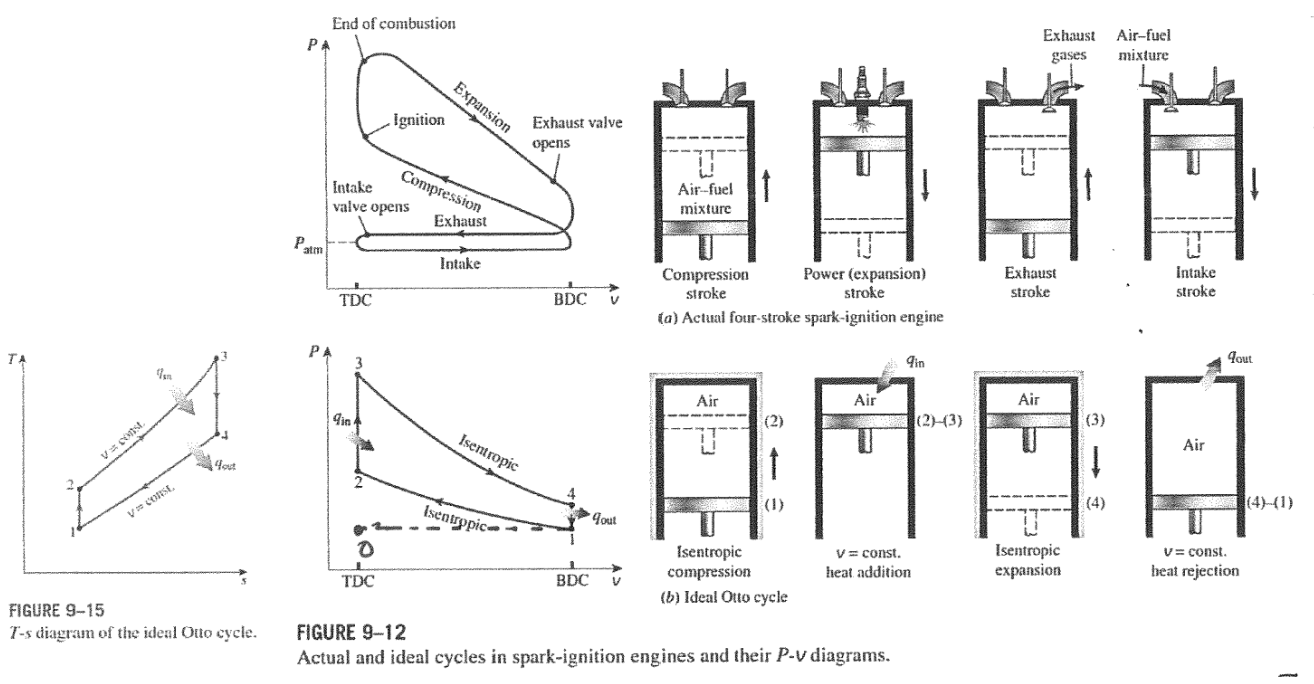
\includegraphics[width = \textwidth]{../img/OttoCycleDiagram}
  \caption{T-S and P-V diagrams for Otto cycle, alongside mechanical cycle breakdown for the ideal and actual cases.} 
\end{figure}
The air-standard Otto cycle is described below in terms of processes.
\begin{itemize}[noitemsep]
  \item Process 1-2: isentropic compression.
  \item Process 2-3: constant volume heat addition.
  \item Process 3-4: isentropic expansion.
  \item Process 4-1: constant volume heat removal
\end{itemize}
In these diagrams, the Otto cycle replaces the combustion process of the actual engine operation with the constant - volume heat addition process. The constant-volume heat removal process replaces the exhaust blowdown. The original figure of the P-V diagram only shows two strokes of the engine. The intake and exhaust strokes are the missing ones. That is accounted for by drawing the graph with a process 0-1 added (the blue line).
\subsection{Efficiency of the Otto cycles}
Lets apply the first law to an Otto cycle during each process separately:
\begin{align}
  \Delta U &= \Delta Q + \Delta W \textrm{ assuming } \Delta PE = \Delta KE \approx 0\\
  \Delta u &= \Delta q + \delta w\\
  \Delta u &= (q_{in} - q_{out}) + (w_{in} - w_{out})
\end{align}
For the heat transfer processes (process 2-3 and process 4-1), $\Delta w = 0$ as there is no boundary work as it is a constant volume process. Therefore for process 4-1 and 2-3:
\begin{equation}
  \Delta u = q_{in} - q_{out}
\end{equation}
For process 4-1: heat removal
\begin{align}
  \Delta u &= -q_{out}\\
  u_1 - u_4 &= - q_{out}\\
  q_{out} &= u_4 - u_1\\
  q_{out} &= c_V(T_4 - T_1)
\end{align}
For process 2-3: heat addition
\begin{align}
  \Delta u &= q_{in}\\
  q_{in} &= u_3 - u_2\\
  q_{in} &= c_V(T_3 - T_2)\\
  \therefore \eta_{th , \ otto} = \frac{w_{net}}{q_{in}} = 1 - \frac{q_{out}}{q_{in}} &= 1 - \frac{T_4 - T_1}{T_3 - T_2} = 1 - \frac{T_4 \left( \frac{T_4}{T_1} -1 \right)}{T_3 \left( \frac{T_3}{T_4} - 1 \right)}
\end{align}
But processes 1-2 and 3-4 are isentropic (adiabatic, internally reversible) and $v_2 = v_3$ and $v_4 = v_1$. From the definition of adiabatic processes:
\begin{align}
  \frac{T_1}{T_2} &= \left( \frac{v_2}{v_1} \right)^{\gamma -1}\\
  \frac{T_4}{T_3} &= \left( \frac{v_3}{v_4} \right)^{\gamma -1}\\
  \therefore \frac{T_1}{T_2} &= \frac{T_4}{T_3}\\
  \therefore \eta-{th, \ otto} &= 1 - \frac{T_4 \left( \frac{T_4}{T_1} -1 \right)}{T_3 \left( \frac{T_3}{T_4} - 1 \right)}\\
  \eta_{th, \ otto} &= 1 - \frac{T_3}{T_4}\left[ \frac{\frac{T_4}{T_3} \frac{T_3}{T_2} \frac{T_2}{T_1} - 1}{\frac{T_3}{T_2} -1} \right]
\end{align}
The compression ratio r is
\begin{equation}
  r = \frac{V_{max}}{V_{min}} = \frac{V_1}{V_2} = \frac{V_4}{V_3}
\end{equation}
Since it is a fixed mass:
\begin{equation}
  r = \frac{v_1}{v_2} = \frac{v_4}{v_3}
\end{equation}
Remember process 2-3 and 4-1  are constant volume processes. Hence, 
\begin{align}
  Pv &= mRt\\
  \frac{v}{mR} &= \frac{T}{P}\\
  \therefore \frac{T_2}{P_2} &= \frac{T_3}{P_3} \rightarrow \frac{P_3}{P_2} = \frac{T_3}{T_2} \textrm{ and}\\
  \therefore \frac{T_4}{P_4} &= \frac{T_1}{P_1} \rightarrow \frac{P_1}{P_4} = \frac{T_1}{T_4}
\end{align}
Process 1-2 and 3-4 are adiabatic (isentropic):
\begin{align}
  Pv &= mRT\\
  \frac{Pv}{T} &= \textrm{constant}\\
  \therefore \frac{P_1 v_1}{T_1} &= \frac{P_2 v_2}{T_2}\\
  \frac{P_2}{P_1} &= \frac{T_2 v_1}{T_1 v_2}\\
  \frac{T_2}{T_1} &= \frac{P_2}{P_1} \cdot \frac{v_2}{v_1}\\
  \frac{T_2}{T_1} &= \frac{P_2}{P_1} \cdot r^{-1}
\end{align} 
Similarly,
\begin{align}
  Pv &= mRT\\
  \frac{Pv}{T} &= \textrm{constant}\\
  \therefore \frac{P_4 v_4}{T_4} &= \frac{P_3 v_3}{T_3}\\
  \frac{P_4}{P_3} &= \frac{T_4 v_3}{T_3 v_4}\\
  \frac{T_3}{T_4} &= \frac{P_3}{P_4} \cdot \frac{v_3}{v_4}\\
  \frac{T_3}{T_4} &= \frac{P_3}{P_4} \cdot r
\end{align} 
Hence,
\begin{align}
  \eta_{th, \ otto} &= 1 - \frac{T_4}{T_3}\left[ \frac{\frac{T_3}{T_2}- 1}{\frac{T_3}{T_2} -1} \right]\\
  \eta_{th, \ otto} &= 1 - \frac{T_4}{T_3}\\
  \eta_{th, \ otto} &= 1 - \left( \frac{1}{r} \right)^{\gamma -1}\\
  \eta_{th, \ otto} &= 1 - \frac{1}{r^{\gamma -1}}\\
  \textrm{where } r &= \frac{v_1}{v_2} = \frac{v_4}{v_3}
\end{align}
\begin{figure}
  \centering
  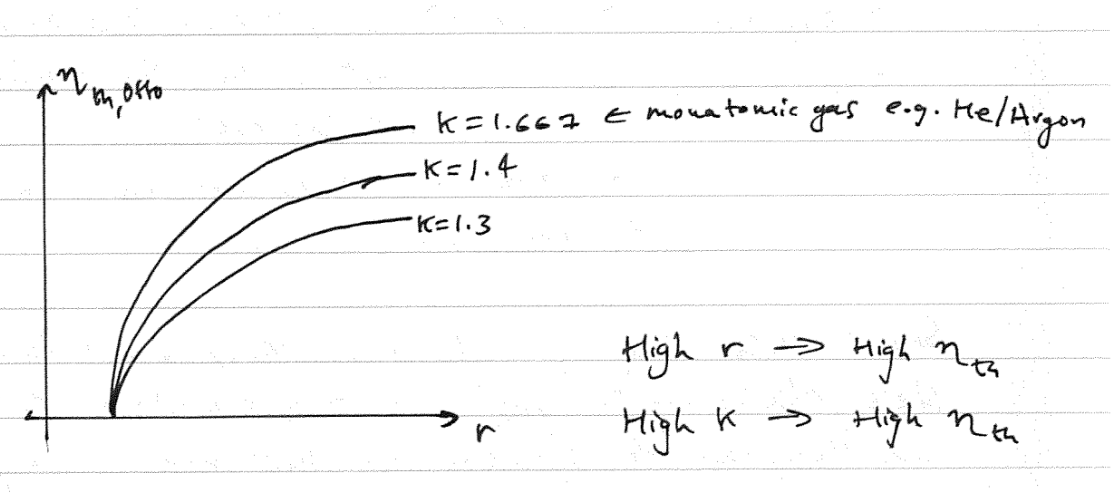
\includegraphics[width = \textwidth]{../img/OttoThermoEfficiency}
  \caption{Graph to show $r$ against $\eta_{th , \ otto}$.}
\end{figure}
For higher efficiency, higher compression ratios are required. However, increase in pressure ratios would increase the air-fuel temperature above the temperature at which the mixture can auto-ignite. This would result in \emph{'engine knock'} (auto ignition that occurs prematurely, produces an audible noise) reducing the performance of the engine. In order to avoid such situations, additives are generally added which increase the auto-ignition temperature.
\subsection{Diesel cycle: ideal cycle for CI engines}
The diesel cycle is the ideal cycle for CI reciprocating engines. It differs to SI engines mainly in the method of initiating combustion.

SI engines have an air-fuel mixture which is compressed below auto-ignition temperature and ignited with a spark. CI engines compress air to a temperature greater than the auto-ignition temperature of the fuel. Fuel is injected into hot compressed air and combustion is initiated. 

Since in diesel engines, only air is compressed during the compression stroke, eliminating the possibility of auto-ignition. Therefore, diesel engines are designed to operate on much higher compression ratios.
\begin{figure}
  \centering
  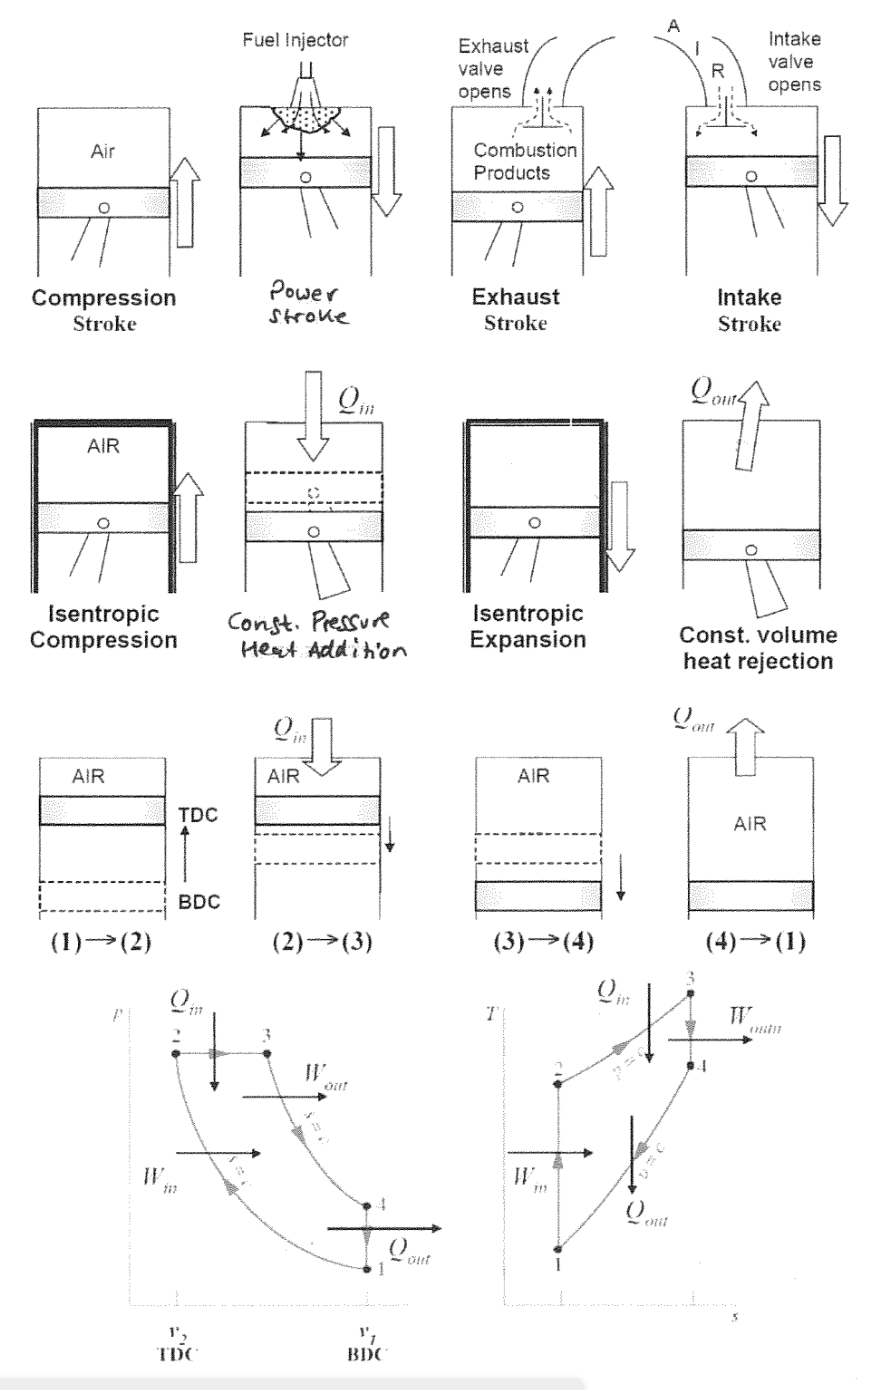
\includegraphics[width = 0.8 \textwidth]{../img/DieselCycleDiagram}
  \caption{Diagram showing mechanical positions of piston at each process step along with P-v and T-s diagrams}
\end{figure}
Assumptions for Diesel cycle.
\begin{itemize}[noitemsep]
  \item Fixed amount of air (ideal gas) for working fluid.
  \item Combustion process replace by constant pressure heat addition.
  \item Intake and exhaust not considered, cycle completed with constant volume heat removal with piston at BDC.
  \item All processes considered internally reversible.
\end{itemize}
The air-standard Diesel cycle is described below in terms of processes.
\begin{itemize}[noitemsep]
  \item Process 1-2: isentropic compression.
  \item Process 2-3: isobaric heat addition.
  \item Process 3-4: isentropic expansion.
  \item Process 4-1: isochoric heat removal.
\end{itemize}
Lets apply the first law to a diesel cycle during each process separately.
\begin{equation}
  \Delta u = (q_{in} - q_{out}) + (w_{in}- w_{out})
\end{equation}
For process 2-3: constant pressure heat addition.
\begin{align}
  u_3 - u_2 &= q_{in} - w_{b, \ out}\\
  q_{in} &= u_3 - u_2 + \int_2^3 P dv\\
  q_{in} &= u_3 - u_2 + P_2 (v_3 - v_2)\\
  q_{in} &= h_3 - h_2\\
  q_{in} &= c_P (T_3 - T_2)
\end{align}
For process 4-1: isochoric heat rejection.
\begin{align}
  u_1 - u_4 &= - q_{out}\\
  q_{out} &= u_4 - u_1\\
  q_{out} &= c_V (T_4 - T_1)
\end{align}
\begin{figure}
  \centering
  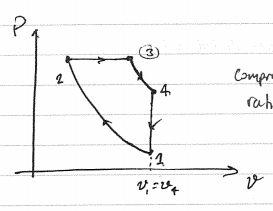
\includegraphics[width = 0.6\textwidth]{../img/PVDiesel}
  \caption{PV diagram for Diesel cycle.}
\end{figure}
Given,
\begin{align}
  \textrm{Compression ratio} \rightarrow r_v &= \frac{v_1}{v_2}\\
  \textrm{Expansion ratio} \rightarrow r_e &= \frac{v_4}{v_3}\\
  \textrm{Cut off ratio} \rightarrow r_c &= \frac{v_3}{v_2}\\
  r_e \cdot r_c = \frac{v_4}{v_3} \cdot \frac{v_3}{v_2} &= \frac{v_4}{V_2} = \frac{v_1}{v_2} = r_v\\
  \therefore r_v &= r_c \cdot r_e
\end{align}
Process 1-2: isentropic compression.
\begin{align}
  \textrm{adiabatic, hence } \frac{T_1}{T_2} = \left( \frac{V_2}{V_1} \right)^{\gamma -1} &= \frac{1}{r_V^{\gamma - 1}}\\
  T_1 &= \frac{T_2}{r_V^{\gamma - 1}} \label{diesel12}
\end{align}
Process 2-3: isobaric heat addition
\begin{align}
  Pv &= RT\\
  \frac{P}{R} &= \frac{T}{v} = \textrm{constant}\\
  \frac{T_2}{v_2} &= \frac{T_3}{v_3}\\
  \therefore T_2 &= T_3 \frac{v_2}{v_3}\\
  T_2 &= \frac{T_3}{v_c} \label{diesel23}
\end{align}
Process 3-4: isentropic heat expansion.
\begin{align}
  \frac{T_4}{T_3} &= \left( \frac{v_3}{v_4} \right)^{\gamma -1} = \frac{1}{r_e^{\gamma -1}}\\
  T_4 &= \frac{T_3}{r_e^{\gamma -1}} \label{diesel34}
\end{align}
Thermal efficiency can be calculated as,
\begin{equation}
  \eta_{th, \ diesel} = 1 - \frac{1}{\gamma} \frac{1}{r_v^{\gamma -1}} \left[ \frac{r_c^{\gamma -1}}{r_c - 1} \right]
\end{equation}
\subsection{Otto and Diesel comparison}
\begin{align}
  \eta_{th, \ diesel} &= 1 - \frac{1}{\gamma} \frac{1}{r_v^{\gamma -1}} \left[ \frac{r_c^{\gamma -1}}{r_c - 1} \right]\\
  \eta_{th, \ otto} &= 1 - \frac{1}{r^{\gamma -1}}\\
  \textrm{for } r_v &= \frac{v_1}{v_2} > 1\\
  \frac{1}{\gamma} \left[ \frac{r_c^{\gamma -1}}{r_c - 1} \right] &> 1
\end{align}
Therefore, the efficiency of the diesel cycle is less than that of the Otto cycle for the same compression ratio. However, the advantages of Diesel over petrol engines is that they can operate at higher compression ratios witout auto-igniton.
\begin{equation}
  \eta_{th, \ otto} > \eta_{th, \ diesel}
\end{equation}
Also if $r_c$ decreases, then $\eta_{th, \ diesel}$ increases. When the limiting case of $r_c = 1$ occurs, the quantity in the brackets becomes 1 and hence $\eta_{th, \ diesel} = \eta_{th, \ otto}$.
\subsection{Brayton cycle (Joule cycle)}
The Brayton cycle (Joule cycle) represents the operation of a gas turbine engine.
\begin{figure}
  \centering
  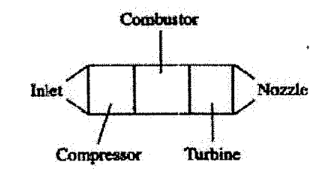
\includegraphics[width = 0.5\textwidth]{../img/Brayton1}
  \caption{Sketch of the jet engine components.}
  \label{brayton1}
\end{figure}
Gas turbines usually operate on an open cycle, as shown in Figure \ref{brayton2}. Fresh air is drawn into the compressor, where its temperature and pressure are. the high-pressure air proceeds into the combistion chamber, where the fuel is burned at constant pressure. The resulting high-temperature gases then enter the turbinem where they expand to the atmospheric pressure while producing ower.  The exhaust gases leaving the turbine are thrown out (not recirculated), causing the cycle to be classified as an open cycle.
\begin{figure}
  \centering
  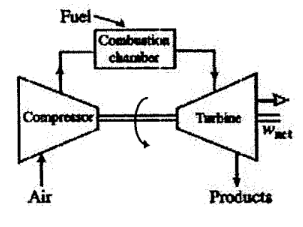
\includegraphics[width = 0.5\textwidth]{../img/Brayton2}
  \caption{Open cycle operation for Joule cycle.}
  \label{brayton2}
\end{figure}
The open gas-turbine cycle described above can be modelled as a closed cycle, as shown in Figure \ref{brayton3}, by utilising the air-standard assumptions. Here the compression and expansion processes remain the samem but the combustion process is replace by a isobaric heat addition process from an external source and the echaust process is replaced bu a isobaric heat rejection process to the ambient air.
\begin{figure}
  \centering
  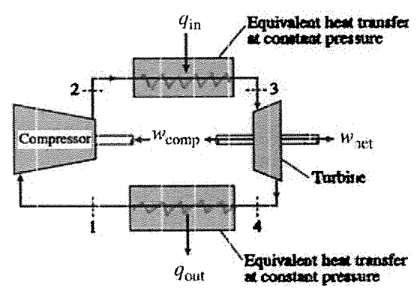
\includegraphics[width = 0.5\textwidth]{../img/Brayton3}
  \caption{Closed cycle operation for Joule cycle.}
  \label{brayton3}
\end{figure}
The ideal cycle that the working fluid undergoes in this closed loop is the Joule cycle. It consists of four processes:
\begin{itemize}[noitemsep]
  \item Process 1-2: isentropic compression in the inlet and compressor.
  \item Process 2-3: isobaric heat addition.
  \item Process 3-4: isentropic expansion, in the turbine and exhaust nozzle, with which we
    \begin{itemize}[noitemsep]
      \item take some work out of the air and use it to drive the compressor and
      \item take the remaining work out and use it to accelerate fluid for jet propulsion, or to turn a generator for electrical power generation.
    \end{itemize}
  \item Process 4-1: isobaric heat rejection.
\end{itemize}
\begin{figure}
  \centering
  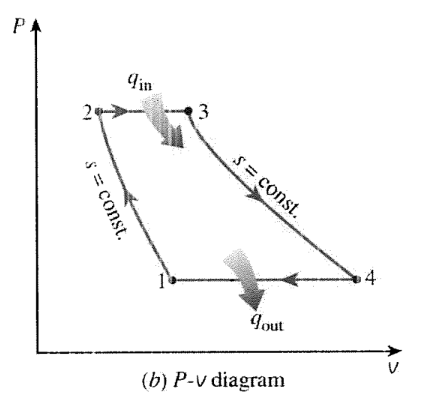
\includegraphics[width = 0.5\textwidth]{../img/BraytonPV}
  \caption{PV diagram for Joule cycle.}
\end{figure}
\begin{figure}
  \centering
  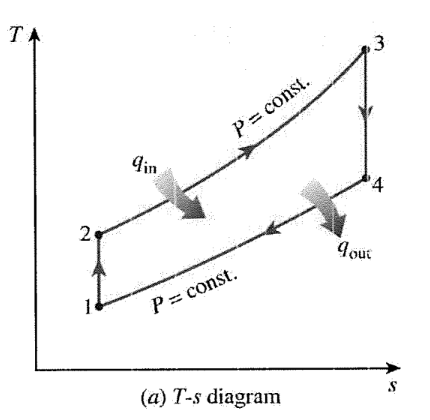
\includegraphics[width = 0.5\textwidth]{../img/BraytonTS}
  \caption{TS diagram for Joule cycle.}
\end{figure}
\subsection{Thermal efficiency of the simple ideal Joule cycle}
\subsubsection{Process 1-2: isentropic compression} 
From the first law, the compressor is a steady flow device, hence let us apply the SFEE:
\begin{equation}
  \frac{dE_{system}}{dt} = [\dot{Q}_{in} + \dot{W}_{in} + \dot{m}_1 (h_1 + \frac{v_1^2}{2} + gz_1) ] - [\dot{Q}_{out} + \dot{W}_{out} + \dot{m}_2 (h_2 + \frac{v_2^2}{2} + gz_2) ]
\end{equation}
Assume steady flow and negligible changes in KE and PE.
\begin{align}
  \dot{W}_{in} + \dot{m}_1 h_1 &= \dot{m}_2 h_2 \ (\dot{m}_1 = \dot{m}_2 = \dot{m})\\
  \dot{W}_{comp} &= \dot{m}(h_2 - h_1)\\
  w_{comp} &= \frac{\dot{W}_{comp}}{\dot{m}}\\
  \frac{\dot{W}_{comp}}{\dot{m}} &= [ w_{comp} = (h_2 - h_1)] \ \si{\kilo\joule\per\kg}
\end{align}
Also, since it is isentropic = adiabatic:
\begin{equation}
  \therefore \frac{T_2}{T_1} = \left( \frac{P_2}{P_1} \right)^{\frac{\gamma - 1}{\gamma}}
\end{equation}
\subsubsection{Process 2-3: isobaric heat addition}
First law: apply SFEE:
\begin{align}
  \dot{Q}_{in} + \dot{m} h_2 &= \dot{m} h_3\\
  \dot{Q}_{in} &= \dot{m} (h_3 - h_2)\\
  q_{in} &= h_3 - h_2 \ \si{\kilo\joule\per\kg}
\end{align}
\subsubsection{Process 3-4: isentropic expression}
First law: apply SFEE:
\begin{align}
  \dot{m} h_3 &= \dot{W}_{turbine} + \dot{m} h_4\\
  \dot{W}_{turbine} &= \dot{m} (h_3 - h_4)\\
  \dot{W}_{turbine} &= h_3 - h_4 \ \si{\kilo\joule\per\kg}
\end{align}
Also, since process 3-4 is isentropic = adiabatic:
\begin{equation}
  \therefore \frac{T_3}{T_4} = \left( \frac{P_3}{P_4} \right)^{\frac{\gamma -1}{\gamma}}
\end{equation}
But $P_2 = P_3$ and $P_1 = P_4$,
\begin{align}
  \therefore \frac{T_3}{T_4} = \left( \frac{P_3}{P_4} \right)^{\frac{\gamma -1}{\gamma}} &= \left( \frac{P_2}{P_1} \right)^{\frac{\gamma -1}{\gamma}} = \frac{T_2}{T_1}\\
  \therefore \frac{T_3}{T_4} &= \frac{T_2}{T_1}
\end{align}
\subsubsection{Process 4-1: isobaric heat rejection}
First law: apply SFEE:
\begin{align}
  \dot{m} h_4 &= \dot{Q}_{out} + \dot{m} h_1\\
  \dot{Q}_{out} &= \dot{m} h_4 - \dot{m} h_1\\
  q_{out} &= h_4 - h_1 \ \si{\kilo\joule\per\kg}
\end{align}
\subsection{Thermal efficiency of Joule cycle}
\begin{gather}
  \eta_{th, \ Joule} = \frac{W_{net}}{Q_{in}} = \frac{w_{net}}{q_{in}} = 1 - \frac{q_{out}}{q_{in}}\\
  \eta_{th, \ Joule} = 1- \frac{T_1}{T_2} = 1 - \left( \frac{P_1}{P_2} \right)^{\frac{\gamma - 1}{\gamma}} = 1 - \left( \frac{V_1}{V_2} \right)^{\gamma -1}
\end{gather}
(as process 1-2 is adiabatic). Also since $r_V = \frac{V_1}{V_2}$ is compression ratio:
\begin{equation}
  \therefore \eta_{th, \ Joule} = 1 - \frac{1}{r_V^{\frac{\gamma -1}{\gamma}}}
\end{equation}
We can also define a new variable, $r_P$, the pressure ratio, where $r_P = \frac{P_2}{P_1}$.
\begin{equation}
  \therefore \eta_{th, \ Joule} = 1 - \frac{1}{r_P^{\frac{\gamma -1}{\gamma}}}
\end{equation}
Thus, the pressure ratio and the value of $\gamma$ determines the thermal efficiency of a Joule cycle. The melting point of the turbine blocks limit the max temperature and thus the pressure ratios that can be used in that cycle (as the maximum temperature in a cycle occurs at the end of the combustion process - state 3). For a fixed turbine inlet temperature $T_3$, the network output per cycle increases within the pressure ratio, reaches a maximum, and then starts to increase. Thus, there should be a compromise between the pressure ratio and the net work output. If net work output per cycle decreases, mass flow rate must increase to produce the same power output. This would require a larger system, which may not be economical.
\begin{figure}
  \centering
  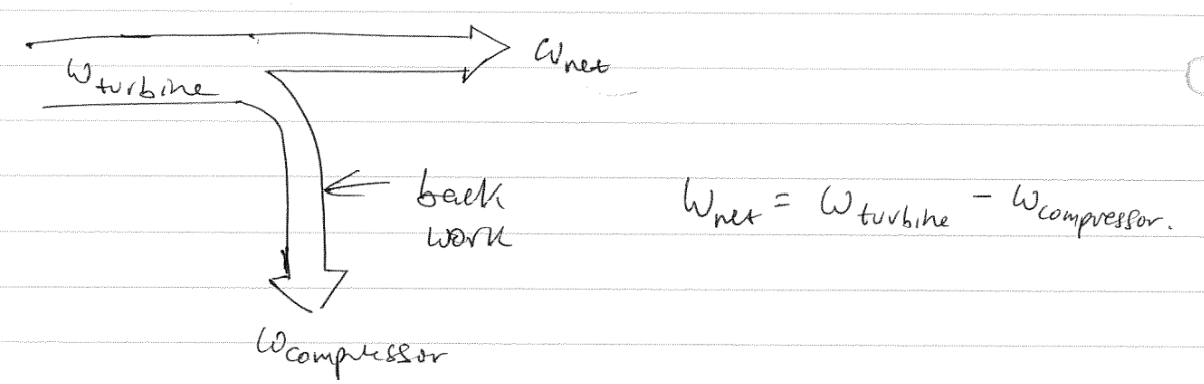
\includegraphics[width = 0.8\textwidth]{../img/JouleCycleDiagram}
  \caption{Diagram of Joule cycle.}
\end{figure}
The ratio of the compressor work to the turbine work is called the back work ratio $= r_{BW}$
\begin{gather}
  \textrm{Back work ratio} = \frac{W_{\textrm{compressor}}}{W_{\textrm{turbine}}} = \frac{h_3 h_1}{h_3 - h_4} = r_{BW}\\
  \textrm{work ratio} = \frac{W_{net}}{W_{\textrm{turbine}}}
\end{gather}
As we showed before, there should be a compromise between the pressure ratio and the net work output. Let us try and work out the value of $T_2$ required for maximum work output when $T-3$ (metallurgical limits) is fixed and $T_1$ (natural sink) is also fixed. 
\begin{align}
  \textrm{net specific work produced} &= W_{\textrm{turbine}} - W_{\textrm{compressor}}\\
  &= (h_3 - h_4) - (h_2 - h_1)\\
  W_{net} &= c_P (T_3 - T_4) - c_P (T_2 - T_1)\\
  \frac{dW_{net}}{dT_2} &= c_P \frac{d}{dT_2} \left[ T_3 - T_4 - T_2 + T_1 \right]\\
  &= c_P \left[ -1 - \frac{dT_4}{dT_2} \right]
\end{align}
Max $W_{net}$ occurs when $\frac{dW_{net}}{dT_2} = 0$
\begin{align}
  \therefore \frac{dW_{net}}{dT_2} &= -1 - \frac{dT_4}{dT_2} = 0\\
  \textrm{from before, } \frac{T_3}{T_4} &= \frac{T_2}{T_1}\\
  T_4 &= \frac{T_1}{T_2}T_3\\
  \therefore -1 - \frac{d}{dT_2} \left[ \frac{1}{T_2} T_1 T_3 \right] &= 0\\
  -1 + \frac{T_1 T_3}{T_2^2} &= 0\\
  T_2 &= \sqrt{T_1 T_3}
\end{align}
For a fixed $T_1$ and $T_3$, $T_2 = \sqrt{T_1 T_3}$ produces the max net work output per unit mass. Also, since:
\begin{equation}
  r_P = \frac{P_2}{P_1} = \left( \frac{T_1}{T_2} \right)^{\frac{\gamma}{1- \gamma}} = \left( \frac{T_2}{T_1} \right)^{\frac{\gamma}{\gamma -1}} 
\end{equation}
For net work output per unit mass to be maximum, $T_2 = \sqrt{T_1 T_3}$. 
\begin{align}
  \therefore r_{P \textrm{ max net work}} &= \left( \frac{\sqrt{T_1 T_3}}{T_1} \right)^{\frac{\gamma}{\gamma -1}}\\
  &= \left( \frac{\sqrt{T_3}}{\sqrt{T_1}} \right)^{\frac{\gamma}{\gamma -1}}\\
  &= \left( \frac{T_3}{T_1} \right)^{\frac{\gamma}{2(\gamma -1)}}
\end{align}
Thus $W_{net, \ max}$ occurs at:
\begin{equation}
  r_P = \left( \frac{T_3}{T_1} \right)^{\frac{\gamma}{2(\gamma -1)}} = \left( \frac{T_{max}}{T_{min}} \right)^{\frac{\gamma}{2(\gamma -1)}}
\end{equation}
\subsection{Derivation of actual gas-turbine cycles from idealised ones}
The actual gas turbine cycle differs from the ideal Joule cycle on several accounts. This occurs because,
\begin{itemize}[noitemsep]
  \item There is a pressure drop from the 'idealised' isobaric heat addition and rejection.
  \item The actual work input to compressor is larger and the actual work output from the turbine is less, due to irreversibilities.
\end{itemize}
The isentropic efficiencies of the turbine and compressor can be used to measure performance. They are expressed as:
\begin{equation}
  \eta_C = \frac{W_s}{W_a} = \frac{\textrm{ideal work}}{\textrm{actual work}} = \frac{h_{2s} - h_1}{h_{2a} - h_1} = \frac{c_P (T_{2s} - T_1)}{c_P (T_2 -T_1)} = \frac{T_{2s} - T_1}{T_2 - T_1}
\end{equation}
\begin{equation}
  \eta_T = \frac{W_a}{W_s} = \frac{\textrm{actual work}}{\textrm{ideal work}} = \frac{h_{3} - h_{4a}}{h_{3} - h_{4s}} = \frac{c_P (T_{3} - T_{4a})}{c_P (T_4 -T_{4s})} = \frac{T_{3} - T_{4a}}{T_4 - T_{4s}}
\end{equation}
\begin{figure}
  \centering
  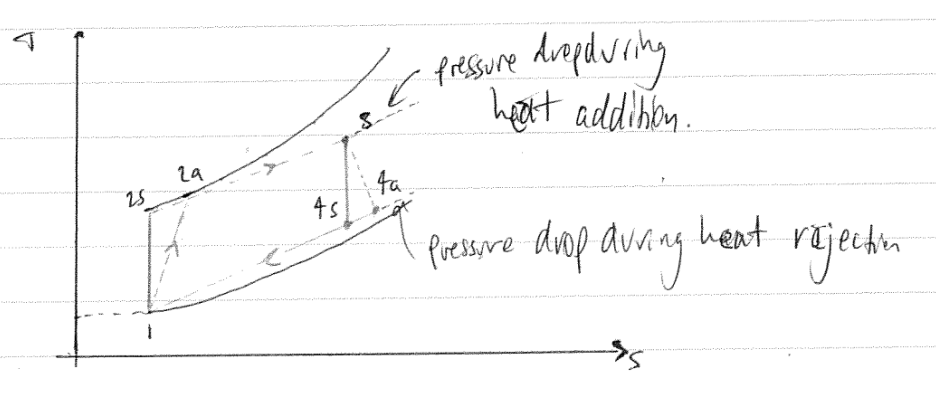
\includegraphics[width = 0.9\textwidth]{../img/efficienciesOfActualJouleCycles}
  \caption{TS diagram of an actual Joule cycle.}
\end{figure}
\end{document}